\documentclass[10pt,twocolumn,letterpaper]{article}

\usepackage{cvpr}
\usepackage{times}
\usepackage{epsfig}
\usepackage{graphicx}
\usepackage{amsmath}
\usepackage{amssymb}

% Include other packages here, before hyperref.

% If you comment hyperref and then uncomment it, you should delete
% egpaper.aux before re-running latex.  (Or just hit 'q' on the first latex
% run, let it finish, and you should be clear).
\usepackage[pagebackref=true,breaklinks=true,letterpaper=true,colorlinks,bookmarks=false]{hyperref}

\cvprfinalcopy % *** Uncomment this line for the final submission

\def\cvprPaperID{****} % *** Enter the CVPR Paper ID here
\def\httilde{\mbox{\tt\raisebox{-.5ex}{\symbol{126}}}}

% Pages are numbered in submission mode, and unnumbered in camera-ready
\ifcvprfinal\pagestyle{empty}\fi
\begin{document}

%%%%%%%%% TITLE
\title{Project Report : CS 7643}

\author{Saheon Kim*, Yuemin Zhou*, and Brandon Sheffield*\\
Georgia Institute of Technology\\
{\tt\small \{skim935,yzhou43,bsheffield7\}@gatech.edu}
% For a paper whose authors are all at the same institution,
% omit the following lines up until the closing ``}''.
% Additional authors and addresses can be added with ``\and'',
% just like the second author.
% To save space, use either the email address or home page, not both
%\and
%Second Author\\
%Institution2\\
%First line of institution2 address\\
%{\tt\small secondauthor@i2.org}
}

\maketitle
%\thispagestyle{empty}

%%%%%%%%% ABSTRACT
\begin{abstract}


   Transformers have disrupted natural language processing and have made their way into computer vision where the Convolutional Neural Network have reigned king for the last decade. In this group project report, we compare dense pixel prediction tasks such as object detection and semantic segmentation performance on the Coco 2017 data set using limited computational resources. We also propose enhancements to the Swin Transformer architecture inspired by recent work done by Meta.

\end{abstract}

%%%%%%%%% BODY TEXT
\section{Introduction/Background/Motivation}

\footnote{Random order. Authors made equal contributions.}

(5 points) What did you try to do? What problem did you try to solve? Articulate your objectives using absolutely no jargon.


We want to test the performance of different architectures in the MMdetection model library against each other. They are specifically Faster RCNN, mask RCNN and Swin transformers. We also want to test the performance of some of these models with compressed images. 


Transformer architectures\cite{vaswani2017attention} have made breakthroughs in natural language processing (NLP). Inspired by the general learning architecture of transformers, vision transformers were introduced as a competitive architecture for computer vision tasks such as image classification\cite{dosovitskiy2020image} with reliance on large-scale pre-training in 2020. There has been an explosion in transformer-based computer vision models with applications ranging from image retrieval\cite{el2021training}, object detection\cite{liu2021swin}, semantic segmentation\cite{wang2021pyramid}\cite{zhang2021multi}\cite{https://doi.org/10.48550/arxiv.2012.15840}, and video understanding\cite{https://doi.org/10.48550/arxiv.2103.15691}\cite{bertasius2021space}\cite{https://doi.org/10.48550/arxiv.2104.11227} have also shown promising results. Motivated by the success of visual transformers, self-supervised methods using vision transformers have been studied showing better results when self-training is applied as opposed to pre-training\cite{zoph2020rethinking}\cite{https://doi.org/10.48550/arxiv.2104.14294}.

Shortly after the introduction of the ViTs that showed to achieve comparable or even superior performance on image classification tasks, the Google Brain team analyzed how ViTs are solving these tasks and how do their learned representations compare to CNNs\cite{raghu2021vision}. Their findings discovered that ViTs with CLS tokens show strong preservation of spatial information which is useful in other computer vision tasks such as object detection. Since then, transformers have made their way into object detection setting key milestones\cite{arkin2021survey}:

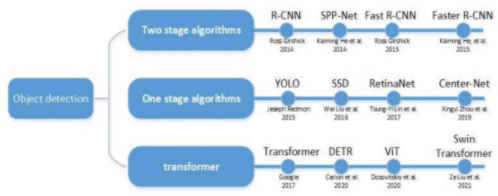
\includegraphics[width=0.8\linewidth]{docs/latex/images/ObjectDetection.png}
\caption{Fig. 1 Object Detection algorithm milestones}


However vision transformers require vasts amount of data, time, and computational memory due to the quadratic cost of self-attention that is dependent on the number of patches. In object detection and segmentation tasks, a $wxh$ image has a complexity of $O(w^2h^2)$ when the images are high-resolution images. An active area of research is scaling down the amount of data and discovering efficient training for visual transformers\cite{liu2021efficient}\cite{lee2021vision}. Furthermore, the amount of labeled data for supervised learning visual transformers poses a challenge for everyone. This challenges motivates advancements in unlabeled data approaches such as self-supervised learning where there has been many exciting advancements in self-supervised visual representation learning  \cite{chen2020simple} \cite{he2020momentum} \cite{henaff2020dat} \cite{chen2020improved} \cite{caron2020unsupervised} \cite{grill2020bootstrap}.

Inspired by the recent work in self-supervised vision transformers\cite{caron2021emerging}, we demonstrate our experimental results on vision transformers with no labeled data for object detection tasks. Object detection is of importance to advancement in automated driving technology therefore we leverage data sets of images captured from the point of view of vehicles such as Kitti\cite{Geiger2012CVPR}, Nuscenes\cite{nuscenes2019}, and Waymo. How well do these techniques work in constrained computational environments where the data sets are small and the hardware resources limit learning?

(5 points) How is it done today, and what are the limits of current practice?

Faster RCNN as a baseline, Mask RCNN as an improvement and SWIN transformer as a further improvement? 

Convolutional Neural Networks(CNNs) have seen an explosion of success in computer vision tasks. CNNs are known to exhibit inductive biases that make them adept at analyzing images for examples. Such inductive biases include: locality, translation equivariance, and translation invariance. These strengths can also be seen as limitations when compared to a ViT that has a more general type of architecture with fewer inductive biases. One limitation is that a CNN is restricted to viewing local features during the early layers of the network. Global features can only be observed when multiple convolutional layers are stacked. However ViTs have global feature awareness from the beginning. ViTs do have notable downsides such as requiring more data to pre-train on.  Additionally in the context of object detection and instance segmentation, ViTs suffer from the quadratic complexity of its self-attention to the image size. As a result, a general-purpose transformer backbone called the Swin Transformer\cite{liu2021swin} was proposed which constructs hierarchical feature maps and has linear computational complexity to image size. It inherits the advantages of the CNN as it fully considers the size invariance and relation between receptive fields. Limitations of the Swin Transformer is that it does not not have as many inductive biases as the CNN such as translation invariance. This in turns make learning very difficult requiring larger datasets and/or stronger data enhancements to achieve better learning performance.

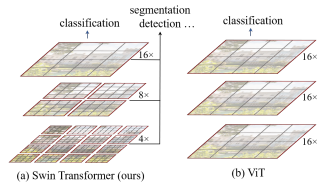
\includegraphics[width=0.8\linewidth]{docs/latex/images/SwinVsViT.png}
\caption{}

Since the introduction of the Swin Transformer in 2020, there has been improvements in regards to scaling up it's capacity and resolution\cite{liu2021swinV2}. Additionally, there have been self-supervised learn methods proposed such as MoBY\cite{xie2021moby} which combines MoCo\cite{he2020momentum}\cite{chen2020improved} with BYOL\cite{grill2020bootstrap} and SimMIM\cite{xie2021simmim} where they use the Swin Transformer backbone.

An enhancement we propose to the Swin Transformer is the use of parallel blocks that results in an architecture that has the same number of parameters and computational complexity while being wider and shallower. This insight was realized while surveying ViTs\cite{touvron2022three} and realized not to exist in Swin Transformer implementations as far as we know.

Given a sequence of transformer blocks:

$x^{'}_{i+1} = x_1 + mhsa_l(x_l)$

$x^{'}_{i+1} = x^{'}_{1+1} + ffn_l(x^{'}_{l+1})$

$x^{'}_{i+2} = x_{1+1} + mhsa_{l+1}(x_{l+1})$

$x_{i+2} = x^{'}_{1+2} + mhsa_{l+1}(x^{'}_{l+2})$


these transformer blocks are combined into two parallel operations:

$x_{l+1} = x_{l} + mhsa_{l,1}(x_l) + mhsa_{l,2}(x_l)$

$x_{l+2} = x_{l+1} + ffn_{l,1}(x_l+1) + ffn_{l,2}(x_{l+1})$

The two parallel operations effectively result in twice the amount of processing that is performed in parallel while reducing the number of layers by two.

(5 points) Who cares? If you are successful, what difference will it make? 

An on-going debate in neural architecture design revolves around balancing width and depth. The first successful neural networks on Imagenet were considered deep in 2014 standards\cite{krizhevsky2012imagenet}\cite{simonyan2014very}. With the introduction of ResNets\cite{he2016deep}\cite{he2016identity} optimization with deep layers suffered due to the residual connections. This deep optimization problem motivated researchers to analyze the trade-offs associated with depth and width\cite{ding2021repvgg}\cite{huang2016deep}\cite{zagoruyko2016wide}. 

There are a number of published works interested in shallower neural networks\cite{goyal2021non}\cite{zagoruyko2016wide} for reasons such as lower latency to easier optimization. One of the simple proposed methods advocates parallel vision transformers\cite{touvron2022three} that takes a sequential architecture and reorganizes the blocks by pairs. The overall result is an architecture that is wider and shallower which is an effective design for more parallel processing, easing optimization, and the reduction of latency dependent on the implementation.

With the rise of attention-based neural networks, wider architectures is once again being revisited\cite{goyal2021non}. In this work "Non-deep Networks", an architecture with several parallel branches is proposed that leads to more complex design. In the work, "Three things everyone should know about Vision Transformers", the authors propose three methods for ViTs that are much simpler and flexible alternative methods: parallel blocks, fine-tuning, patch pre-processing\cite{touvron2022three}. 

We borrow the insight of parallel blocks and adapt it to Swin Transformers\cite{liu2021swin} which is a variant of ViTs.

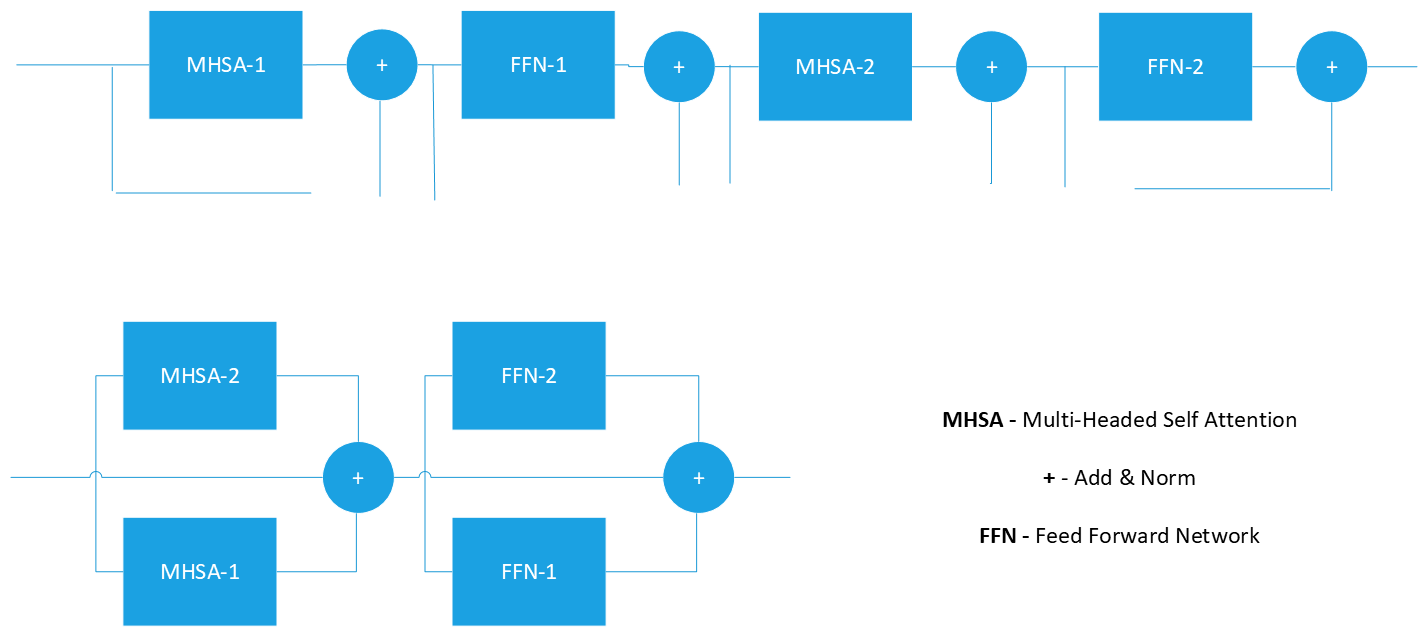
\includegraphics[width=0.8\linewidth]{docs/latex/images/MHSA-Original.png}
\caption{}

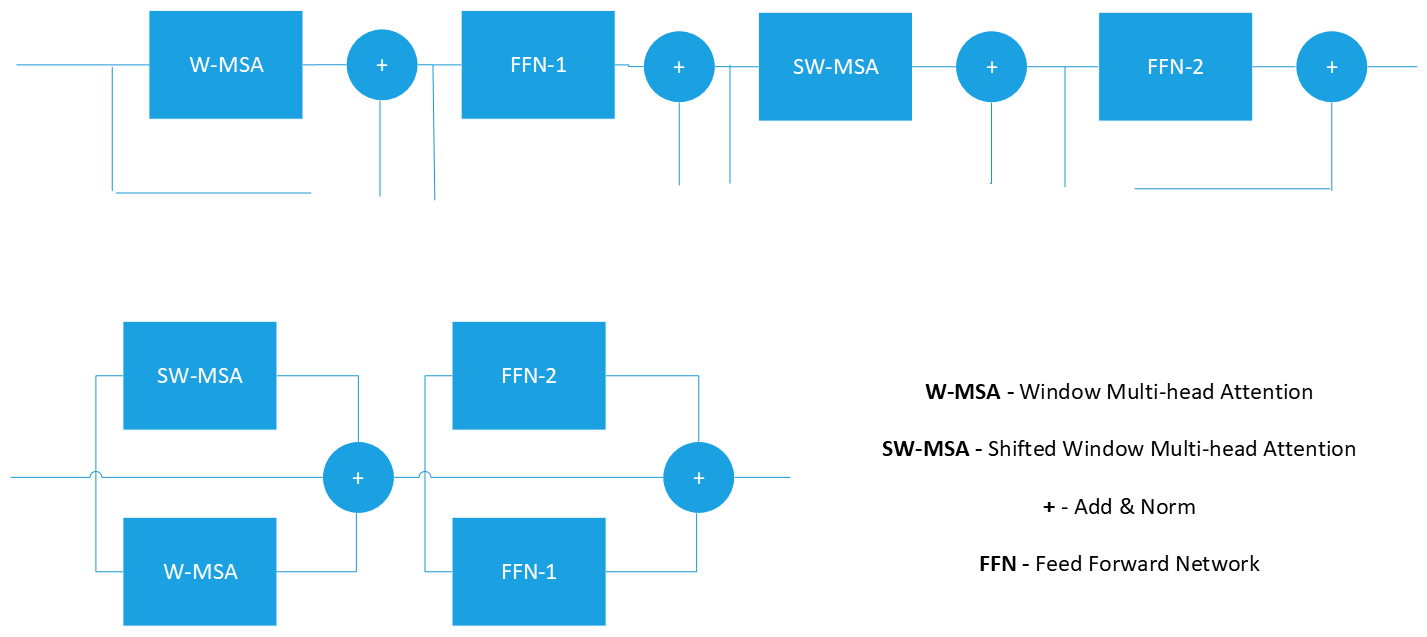
\includegraphics[width=0.8\linewidth]{docs/latex/images/MSA-Swin.png}
\caption{}



(5 points) What data did you use? Provide details about your data, specifically choose the most important aspects of your data mentioned \href{https://arxiv.org/abs/1803.09010}{here}. You don’t have to choose all of them, just the most relevant.


%-------------------------------------------------------------------------
%------------------------------------------------------------------------
\section{Approach}

(10 points) What did you do exactly? How did you solve the problem? Why did you think it would be successful? Is anything new in your approach?

In the context of objection detection tasks, what properties do Swin Transformers introduce to other traditional architectures such as CNNs?


How useful is a self-supervised model for a challenging domain specific use-case: underwater trash or plastic in river

(5 points) What problems did you anticipate? What problems did you encounter? Did the very first thing you tried work?

Visual transformers have an inherit difficulty in requiring lots of hardware resources such as storage and GPUs. For smaller experiments, we utilized local resources such as a NVIDIA RTX 3080ti that has 12GB of memory. Notably the memory of the GPU card has a limiting effect on batch size that is not comparable to results reported in literature. To deal with this limitation, we leveraged free cloud resources by Amazon and Google with \$50 of credit respectively.


There are a number of published works interested in shallower neural networks\cite{goyal2021non}\cite{zagoruyko2016wide} for reasons such as lower latency to easier optimization. One of the simple proposed methods advocates parallel vision transformers\cite{touvron2022three} that takes a sequential architecture and reorganizes the blocks by pairs. The overall result is an architecture that is wider and shallower which is an effective design for more parallel processing, easing optimization, and the reduction of latency dependent on the implementation.

With the rise of attention-based neural networks, wider architectures is once again being revisited\cite{goyal2021non}. In this work "Non-deep Networks", an architecture with several parallel branches is proposed that leads to more complex design. In the work, "Three things everyone should know about Vision Transformers", the authors propose three methods for ViTs that are much simpler and flexible alternative methods: parallel blocks, fine-tuning, patch pre-processing\cite{touvron2022three}.

Here we illustrate the sequential then proposed parallel block methods for ViTs. Given a sequence of transformer blocks:

$x^{'}_{i+1} = x_1 + mhsa_l(x_l)$

$x^{'}_{i+1} = x^{'}_{1+1} + ffn_l(x^{'}_{l+1})$

$x^{'}_{i+2} = x_{1+1} + mhsa_{l+1}(x_{l+1})$

$x_{i+2} = x^{'}_{1+2} + mhsa_{l+1}(x^{'}_{l+2})$

The original authors proposed the following parallel transformer blocks:
>>>>>>> b291d1ff6af9546de459a32d83029d76b7884009

$x_{l+1} = x_{l} + mhsa_{l,1}(x_l) + mhsa_{l,2}(x_l)$

<<<<<<< HEAD
You are welcome to introduce additional sections or subsections, if required, to address the following questions in detail. 
=======
$x_{l+2} = x_{l+1} + ffn_{l,1}(x_l+1) + ffn_{l,2}(x_{l+1})$

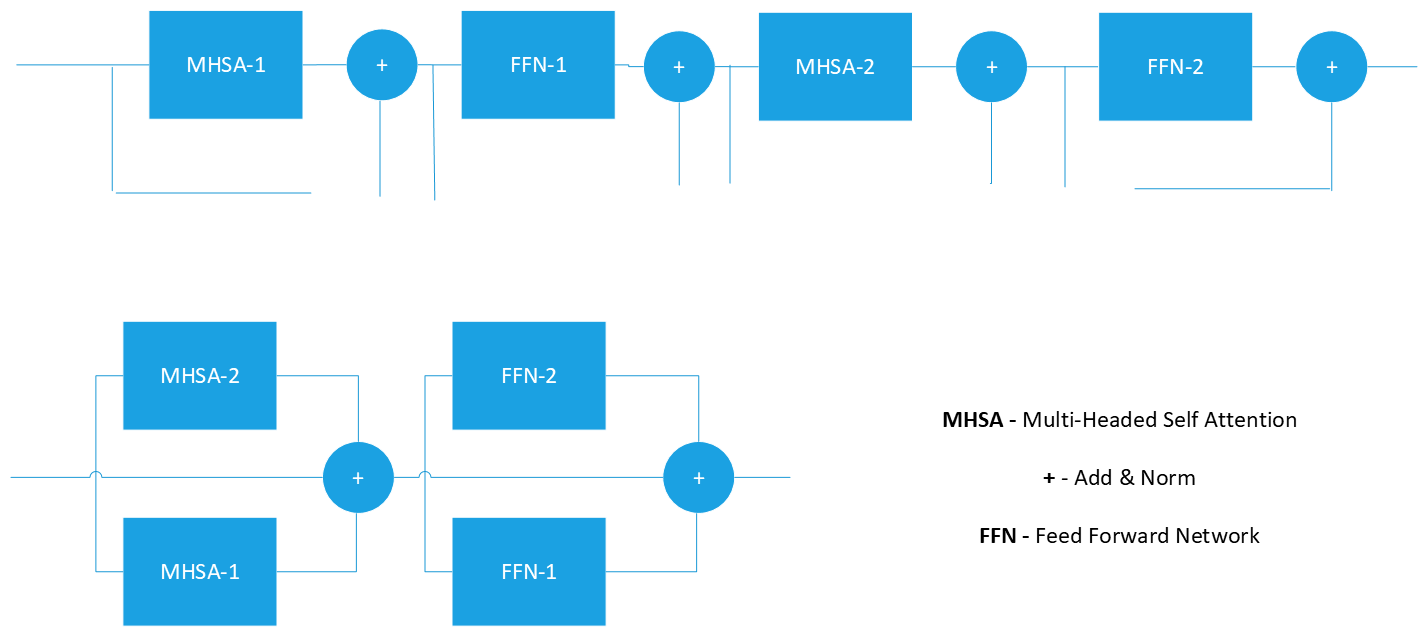
\includegraphics[width=0.8\linewidth]{docs/latex/images/MHSA-Original.png}
\caption{Top - Original sequential attention blocks. Bottom - parallel attention blocks.}
>>>>>>> b291d1ff6af9546de459a32d83029d76b7884009

TODO insert results they found from more breadth than depth

The Swin Transformer is notably a variant of the original ViT therefore there are design changes to consider. For one, the Swin Transformer introduces the ideas of using the regular and shifted windows for computing attention which is not found in classic ViTs. The use of these windows avoids quadratic complexity of global attention with respect to the number of tokens as it would require an intractable amount of tokens for dense prediction tasks as well as computing on high-resolution images. The equations for computing these two windows are as followed:

$\omega(MSA) = 4hwC^2 + 2(hw)^{2}C,$

$\omega(W-MSA) = 4hwC^2 + 2M^{2}hwC,$

These windows can now be placed into the Swin Transformer blocks:

TODO: Fix equations

$z^{l} = W-MSA (LN(z^{l-1})) + z^{l-1}$

$z^{l} = MLP (LN(z^{l})) + z^{l}$

$z^{l+1} = W-MSA (LN(z^{l-1})) + z^{l-1}$

$z^{l+1} = MLP (LN(z^{l+1})) + z^{l+1}$

The insight of parallel blocks can be adapted to Swin Transformers\cite{liu2021swin} which is a variant of ViTs. The original Swin Transformer two block layout is defined as:

$x^{'}_{i+1} = x_1 + mhsa_l(x_l)$

$x^{'}_{i+1} = x^{'}_{1+1} + ffn_l(x^{'}_{l+1})$

$x^{'}_{i+2} = x_{1+1} + mhsa_{l+1}(x_{l+1})$

$x_{i+2} = x^{'}_{1+2} + mhsa_{l+1}(x^{'}_{l+2})$

It can be observed that these two Swin Transformer blocks can also be placed in parallel fashion.

TODO: Fix equations

$x_{l+1} = x_{l} + mhsa_{l,1}(x_l) + mhsa_{l,2}(x_l)$

$x_{l+2} = x_{l+1} + ffn_{l,1}(x_l+1) + ffn_{l,2}(x_{l+1})$

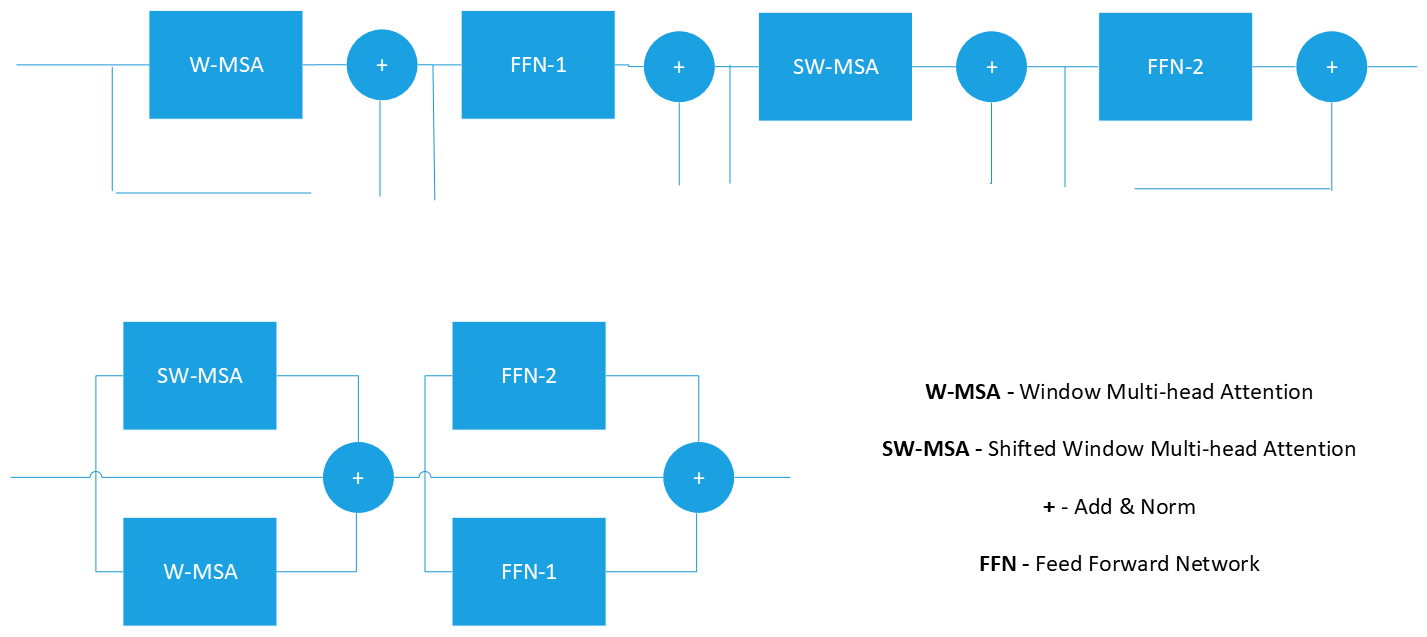
\includegraphics[width=0.8\linewidth]{docs/latex/images/MSA-Swin.png}
\caption{}

(5 points) What data did you use? Provide details about your data, specifically choose the most important aspects of your data mentioned \href{https://arxiv.org/abs/1803.09010}{here}. You don’t have to choose all of them, just the most relevant.

Due to computational limitations and limitations of the models we chose we eventually settled on a truncated version of the coco dataset. This dataset has the bbox annotations and the mask annotations needed for fast RCNN and mask RCNN. This data was further truncated to 1977 images for train, 500 for test, and 494 for validation. These images were all taken from the original training data set. This drastic truncation is needed due to our limited time and computational hardware.  

Also for coco we focused on one class classification because the classes in the dataset was quite imbalanced. 

Insert Coco17 details here

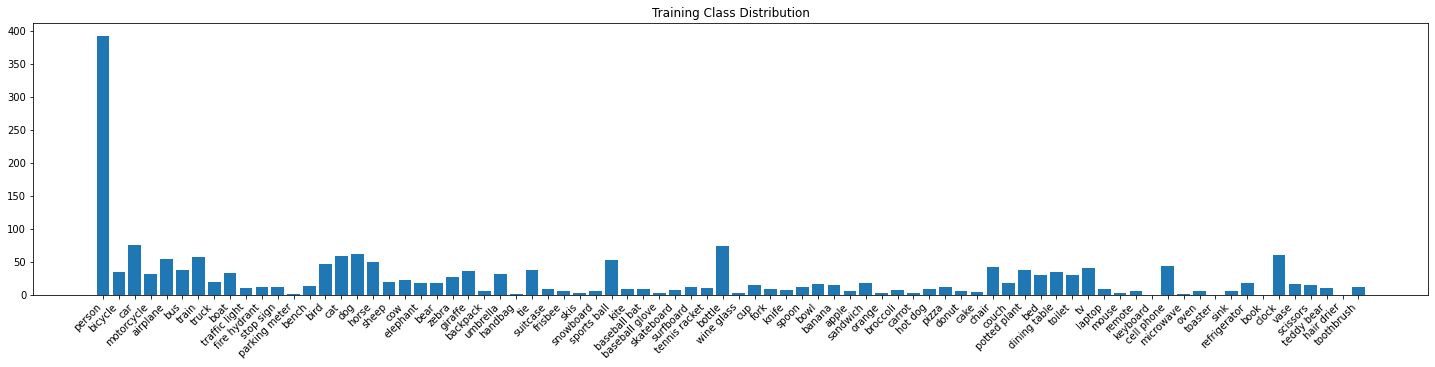
\includegraphics[width=0.8\linewidth]{docs/latex/images/coco17_train_trunc.png}
\caption{}

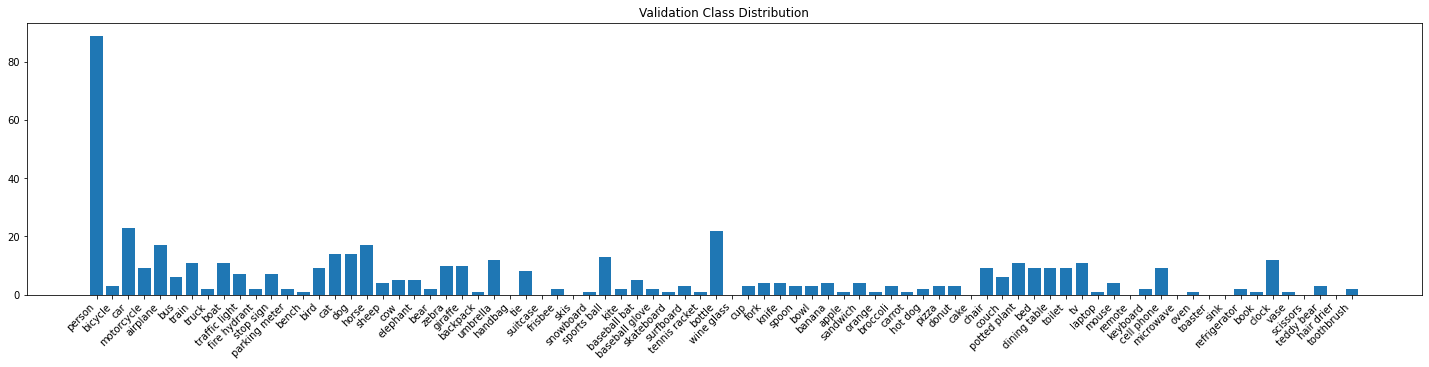
\includegraphics[width=0.8\linewidth]{docs/latex/images/coco17_val_trunc.png}
\caption{}

%-------------------------------------------------------------------------
%------------------------------------------------------------------------
\section{Approach}

(10 points) What did you do exactly? How did you solve the problem? Why did you think it would be successful? Is anything new in your approach?

We demonstrate CNN and Transformer performance on dense pixel prediction tasks independently on the COCO 2017 dataset. A new approach is proposed at the end for Swin Transformers. Experimental results are not provided because of computational constraints.

(5 points) What problems did you anticipate? What problems did you encounter? Did the very first thing you tried work?

The types of architectures that we experimented with and analyzed have an inherit difficulty in requiring lots of hardware resources such as storage and GPUs.

\textbf{Important: Mention any code repositories (with citations) or other sources that you used, and specifically what changes you made to them for your project. }

\section{Experiments and Results}

(10 points) How did you measure success? What experiments were used? What were the results, both quantitative and qualitative? Did you succeed? Did you fail? Why? Justify your reasons with arguments supported by evidence and data.

TODO detail neural network architecture designs
Faster RCNN
The first layer is a CNN layer from resnet. It had four stages. The results of this layer is connected to a neck which is a Feature Pyramid Network. 


TODO comparison of results from coco17

TODO metrics. Examples below

https://github.com/open-mmlab/mmdetection/blob/master/docs/en/useful_tools.md

Metrics: FPS Benchmark, Robust Detection

Confusion Matrix

Model Complexity in FLOPs and params

Error Analysis

Results Analysis

Log Analysis


\textbf{Important: This section should be rigorous and thorough. Present detailed information about decision you made, why you made them, and any evidence/experimentation to back them up. This is especially true if you leveraged existing architectures, pre-trained models, and code (i.e. do not just show results of fine-tuning a pre-trained model without any analysis, claims/evidence, and conclusions, as that tends to not make a strong project). }

\section{Experiences}


\subsection{Challenges}

We first proposed a group project on detecting 3D objects from point cloud data. It was obvious to us that the topic was a hot research area with the motivation of self-driving applications at the wheel. However, once the team became hands-on with the point cloud data, it became apparent that interprability and specialized tools required to interpret sparse point cloud data was not as natural as typical camera images. We then changed topics to more relatable material covered in class such as CNNs and transforms from NLP while staying consistent with object detection.

\subsection{New Challenges}

Whether processing point cloud data or camera images with recent methods, computational resources such as access to enterprise GPUs would always prove to be a challenge. Training on large datasets requires large batch sizes affecting training time and model performance.

\subsection{Team Achievements}

Although the computational resources were out of reach for the team using Colab and local GPU resources, we effectively learned about bleeding edge research topics in computer vision that are actively being improved and published on. For example, ViTs have a new workshop at CVPR 2022 since their introduction in 2020. Also the Swin Transformer won the ICCV 2021 best paper award. There has also been a published Swin Transformer v2 and complementary SimMIM that have been accepted for ICCV 2022. We see this exposure as an advantage for collaboration and future work with prospective research teams from the private and public sectors.

%-------------------------------------------------------------------------
\section{Other Sections}

You are welcome to introduce additional sections or subsections, if required, to address the following questions in detail. 

(5 points) Appropriate use of figures / tables / visualizations. Are the ideas presented with appropriate illustration? Are the results presented clearly; are the important differences illustrated? 

(5 points) Overall clarity. Is the manuscript self-contained? Can a peer who has also taken Deep Learning understand all of the points addressed above? Is sufficient detail provided? 

(5 points) Finally, points will be distributed based on your understanding of how your project relates to Deep Learning. Here are some questions to think about: 

What was the structure of your problem? How did the structure of your model reflect the structure of your problem? 

What parts of your model had learned parameters (e.g., convolution layers) and what parts did not (e.g., post-processing classifier probabilities into decisions)? 

What representations of input and output did the neural network expect? How was the data pre/post-processed?
What was the loss function? 

Did the model overfit? How well did the approach generalize? 

What hyperparameters did the model have? How were they chosen? How did they affect performance? What optimizer was used? 

What Deep Learning framework did you use? 

What existing code or models did you start with and what did those starting points provide? 

Briefly discuss potential future work that the research community could focus on to make improvements in the direction of your project's topic.

\section{Future Work}

Transformers in computer vision is a hot research topic. As of 03/02/2022, the Swin Transformer v2\cite{liu2021swinV2} and SimMIM\cite{xie2021simmim} was accepted by CVRP 2022. The Swin Transformer v2 coupled with SimMIm which is a self-supervised pre-training approached based on masked image model, requires using 40x less labelled data than that of previous billion-scale models based on JFT-3B\cite{dai2021coatnet}\cite{riquelme2021scaling}\cite{https://doi.org/10.48550/arxiv.2106.04560}.

%-------------------------------------------------------------------------

\section{Work Division}

\begin{table*}
\begin{center}
\begin{tabular}{|l|c|p{8cm}|}
\hline
Student Name & Contributed Aspects & Details \\
\hline\hline
Brandon Sheffield & Implementation and Analysis & Trained the Swin Transformer. Implemented parallel blocks to improve results. \\
Saheon Kim & Implementation and Analysis & Trained the  \\
Yuemin Zhou & Implementation and Analysis & Trained the \\
\hline
\end{tabular}
\end{center}
\caption{Contributions of team members.}
\label{tab:contributions}
\end{table*}

\section{Appendices}
\subsection{Code Repositories}
https://github.com/open-mmlab/mmdetection
https://github.com/mastash3ff/cs7643-GroupProject


{\small
\bibliographystyle{ieee_fullname}
\bibliography{egbib}
}
Ren, Shaoqing, et al. “Faster R-CNN: Towards Real-Time Object Detection with Region Proposal Networks.” Arxiv.org, 6 Jan. 2016, https://arxiv.org/pdf/1506.01497.pdf. 

Lin, Tsung-Yi, et al. “Feature Pyramid Networks for Object Detection.” ArXiv.org, 19 Apr. 2017, https://arxiv.org/abs/1612.03144. 

\end{document}
